\mysection{Constructing the System Performance Model}\label{complexSystem}

Usually a system needs more than just one component.
Therefore, a clever way to systematically link all those different components together is needed, as
we want to enable resource sharing, as well as a pipelined stream of data, in the system performance model.
This can be done by aligning multiple resources horizontally and multiple event streams vertically~\cite{wan:06}.

\mysubsection{Flow of Data}

Each event stream is typically processed by a sequence of HW/SW components.
The horizontal order of the steams determines the order, in which the event streams will pass by the resources~\cite{wan:06}.
At every intersection between an event and a resource stream, a component will be instantiated, in case that event stream needs to fulfil a task at this resource.

\mysubsection{Resource Sharing --- Impact of different Scheduling Policies}\label{scheduling}

An important step for designing a real-time embedded system is choosing a scheduling scheme for the resources,
as there are usually several event streams that need to use the same component at one time.
In the framework of MPA, various scheduling and arbitration policies can be used, like for example  
fixed priority, proportional share, TDMA, generalized processor sharing or earliest deadline first scheduling~\cite{wan:06}.
All of these policies have different techniques to distribute the available resources, in particular the remaining service capacities \(\beta'\), among the event streams in need.

Earlier, different approaches were needed when analyzing different classes of arbitration strategies, such as dynamic, static or hierarchical ones, as their event bounds need to be characterized in complete different ways.
Yet since~\cite{slo} there is a unified request bound available for all kinds of analysis purposes in real-time scheduling theory.
Therefore, the response time analysis can now be done with the same unified equation, identically what arbitration strategy is used in the system.

Following there are some examples of common scheduling policies and their uses in MPA.\

\mysubsubsection{Preemptive Fixed Priority Scheduling}

In a system with a fixed priority scheduling strategy, the processor always executes the task with the highest priority of the queue first. 
As those priorities are static, they do not change during execution time.
A preemptive scheduler additionally has a clock and will stop the execution of the task after a certain amount of time units have passed, to put the task back
into the queue and continue with the next one.
Meanwhile, a non-preemptive scheduler does never interrupt the execution of tasks and lets them run until they voluntarily unblock the processor again~\cite{mar}.

In preemptive fixed priority scheduling, tasks are preempted by higher priority tasks~\cite{slo}.
The vertical order of the event streams within the system model determines which event stream will get the highest service capacity and therefore determine the priorities of the event streams~\cite{wan:06}.
In general urgent or highly frequent tasks should be prioritized.
The lower priority event streams below can then only use the remaining service capacity to fulfill their tasks at the same processor~\cite{mar}.
As MPA is especially suitable for modeling fixed priority scheduling, this will be the primary used scheduling technique of the paper.

\mysubsubsection{Non-Preemptive Fixed Priority Scheduling}

Fixed priority scheduling with a non-preemptive strategy can also be used in the framework of MPA, yet
the integration into the system model is more complex than integrating its preemptive equivalent.
However, since~\cite{cho:08} and~\cite{sof:12/1} efficient and sufficiently general approaches are known 
to analyze systems with such arbitration behavior.
Still it is not possibly to just simply use GPUs here, as the components are not supposed to just process all inputs in a greedy manner one after another.
Instead, there is the need for abstracting the scheduling strategy from the system-level components like shown in \autoref{fig:scheduling-unit}.

\begin{figure}
    \centering
    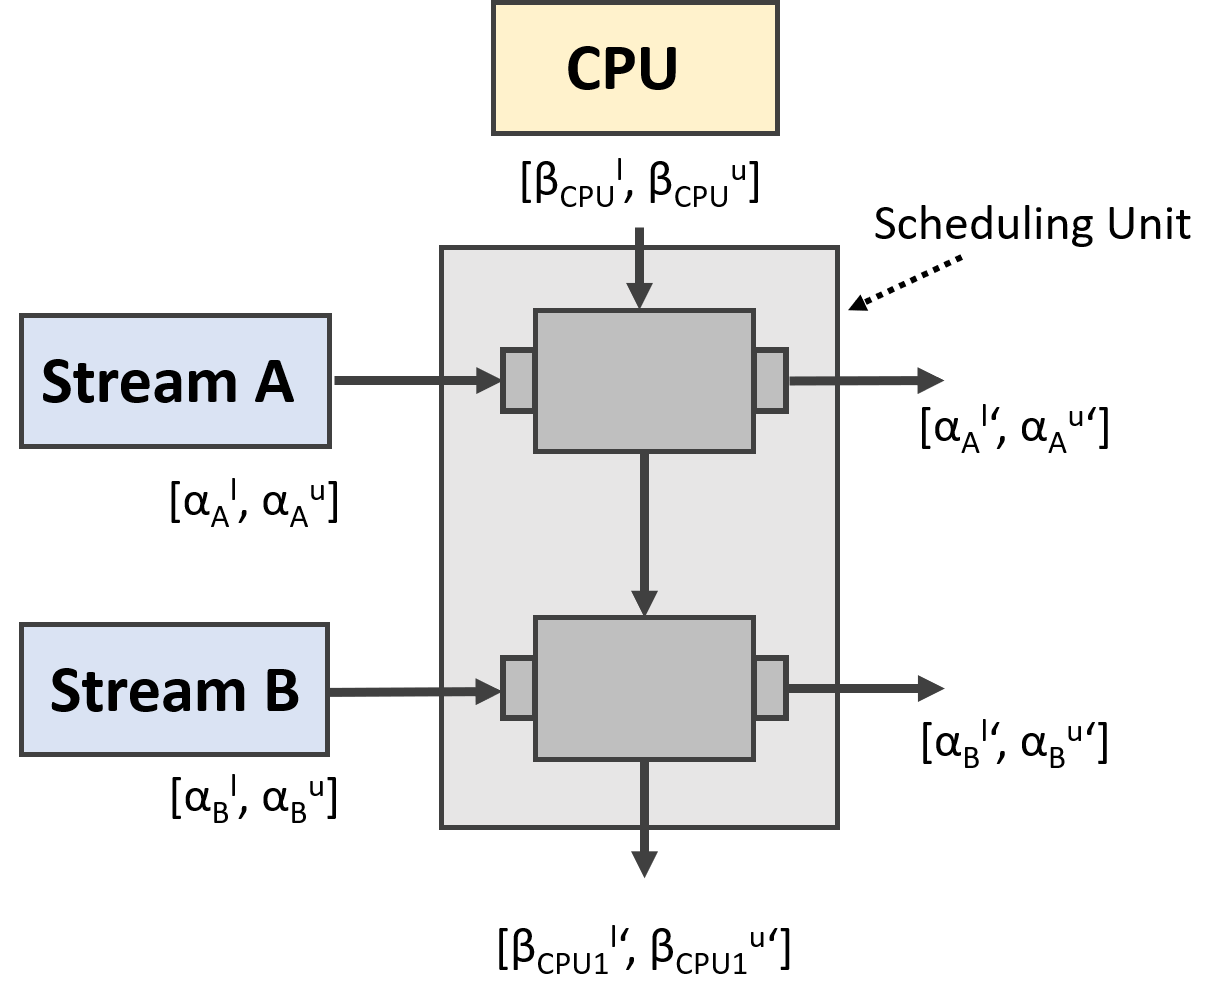
\includegraphics[width=0.8\columnwidth]{graphics/scheduling_unit.png}
    \caption{System Performance Model scheduled using a more complex arbitration technique. This could for example be Fixed Priority Non-Preemptive or Earliest Deadline First Scheduling. %
    The scheduling unit abstracts from the real components and manages what the component will process first.}\label{fig:scheduling-unit}
\end{figure}

\mysubsubsection{Earliest Deadline First Scheduling (\textbf{EDF})}

Similar to non-preemptive fixed priority scheduling, when using EDF scheduling, there is also the need to abstract the arbitration strategy from the components themselves (see \autoref{fig:scheduling-unit}).
Luckily there is great \href{https://www.mpa.ethz.ch/}{tool support} that allows us to treat EDF components just like any ``normal'' GPC.\
However, there now is the need to additionally include the deadline of every task into the calculation.
Using these deadlines, the demand bound function can be specified as the deadline shifted request bound function~\cite{slo}.

\mysubsection{System Performance Model of the Sample System}

Starting with the input data collected in \autoref{data} we can now construct a possible performance model of our system.
Here we decide to actually propose two different models in order to compare them later on: model A with two CPUs of 4 MIPS each connected by a bus (\autoref{fig:system-A}),
as well as model B of only one 5 MIPS CPU (\autoref{fig:system-B}).

After mapping the tasks to their corresponding resources using the information from \autoref{fig:seq_brightness} and \autoref{fig:seq_message}, we define all components to be GPCs.
As a scheduling technique we choose preemptive fixed priority scheduling and give the brightness event stream a higher priority than the
message event stream, as brightness events can occur more often and need quicker processing, in order for the system to seem responsive.

\begin{figure}
    \centering
    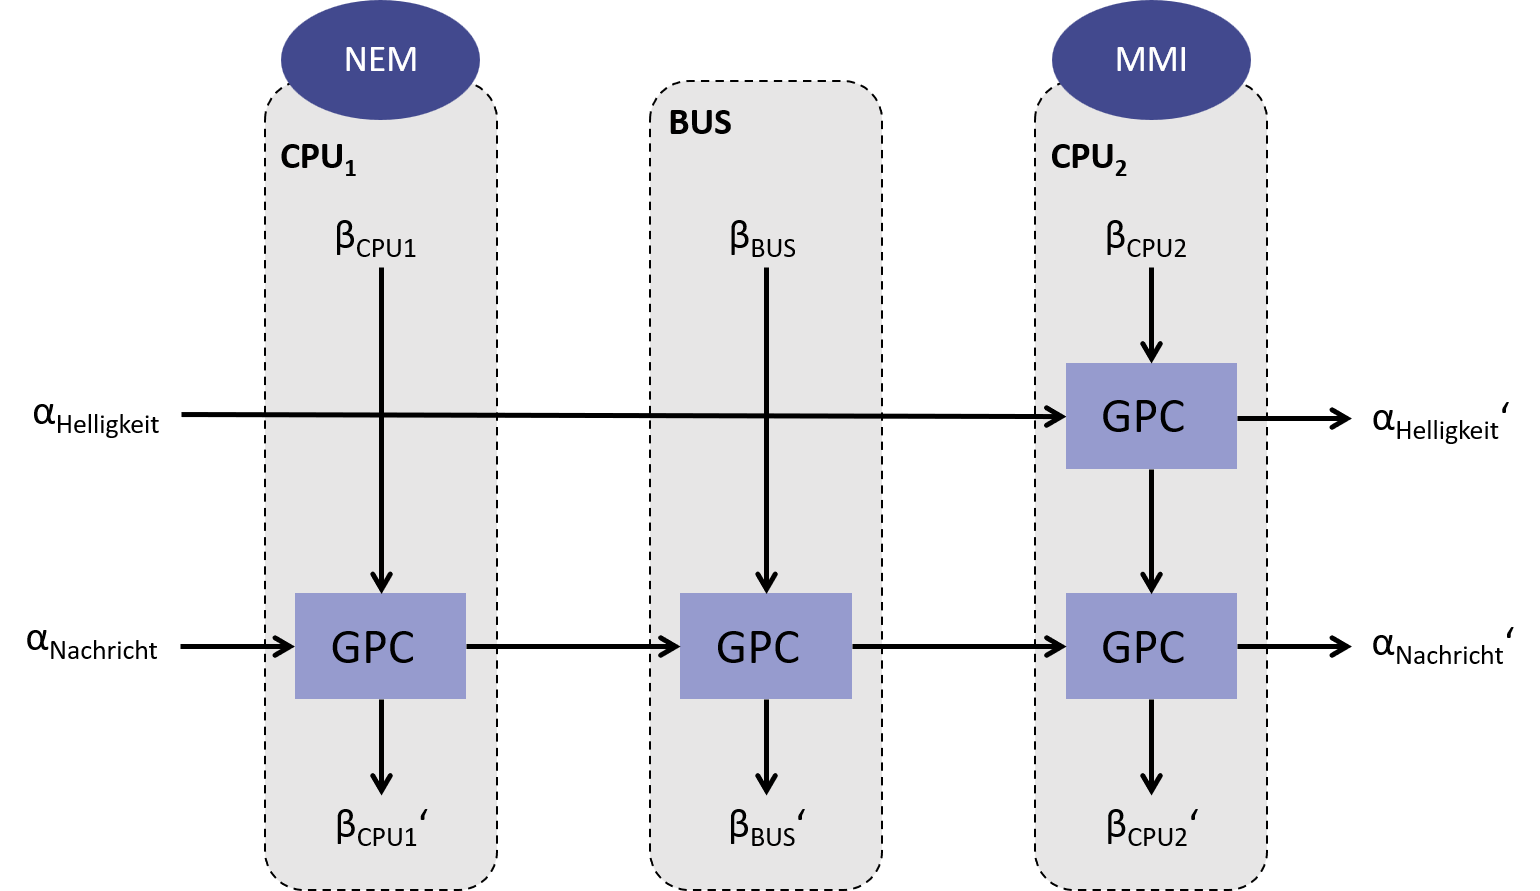
\includegraphics[width=\columnwidth]{graphics/system_A.png}
    \caption{System Performance Model of Architecture A}\label{fig:system-A}
\end{figure}

\begin{figure}
    \centering
    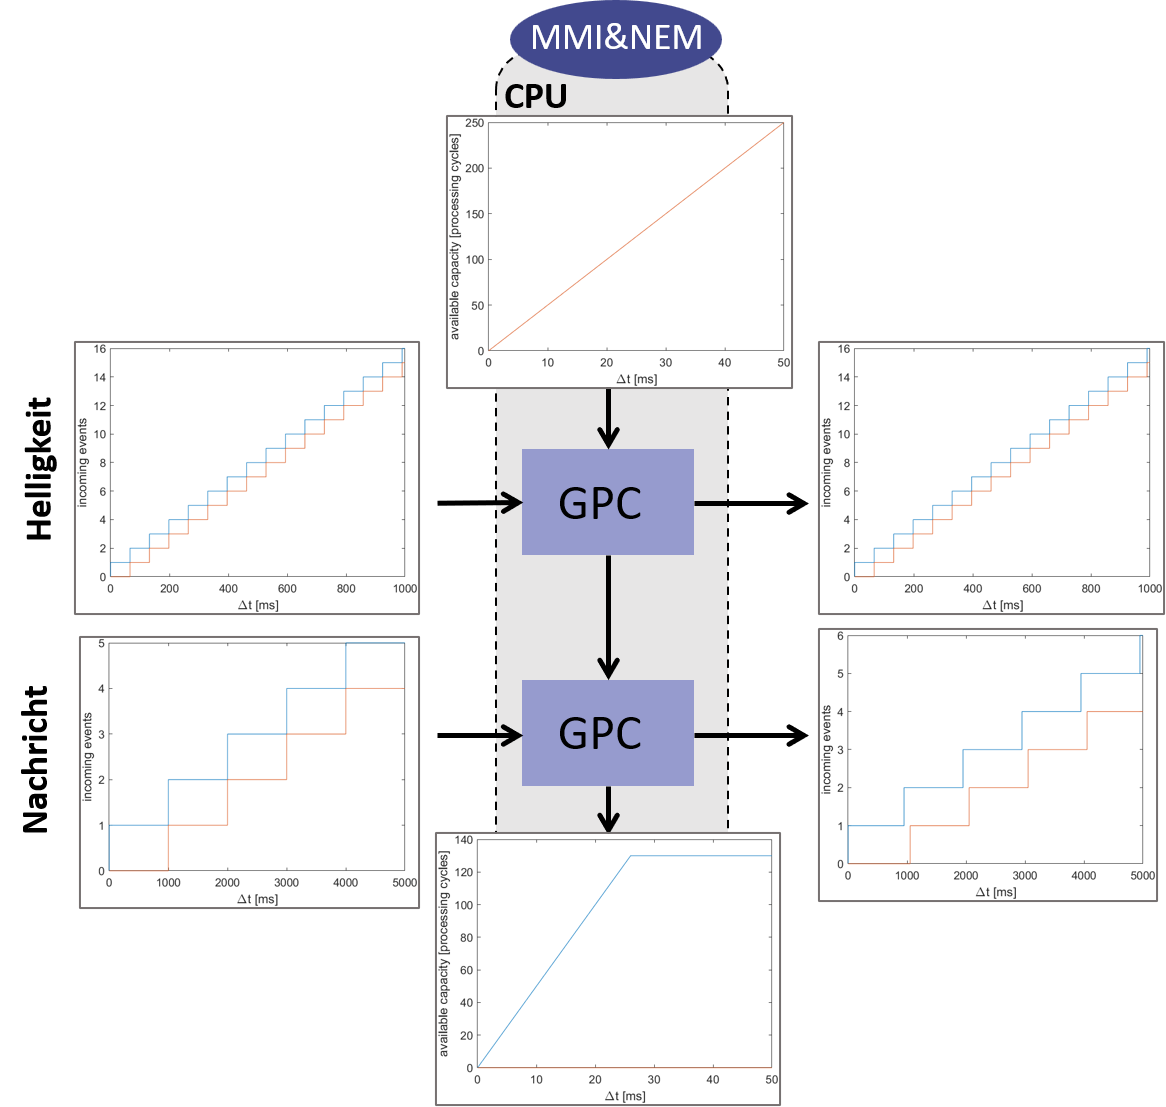
\includegraphics[width=0.9\columnwidth]{graphics/system_B.png}
    \caption{System Performance Model of Architecture A with the plotted input and output streams}\label{fig:system-B}
\end{figure}